\subsection{棱台}\label{subsec:2-3}

\begin{enhancedline}

\subsubsection{棱台的概念和性质}

\begin{wrapfigure}[9]{r}{5.5cm}
    \centering
    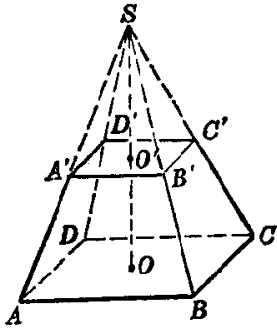
\includegraphics[width=4.5cm]{../pic/ltjh-ch2-20.png}
    \caption{}\label{fig:ltjh-2-20}
\end{wrapfigure}

用一个平行于棱锥底面的平面去截棱锥,底面和截面之间的部分叫做\zhongdian{棱台}。
原棱锥的底面和截面叫做\zhongdian{棱台的下底面}和\zhongdian{上底面},
其他各面叫做\zhongdian{棱台的侧面}。相邻侧面的公共边叫\zhongdian{做棱台的侧棱},
上、下底面之间的距离叫做\zhongdian{棱台的高}。如图 \ref{fig:ltjh-2-20} 中的棱台,
多边形 $A'B'C'D'$ 和 $ABCD$ 是上、下底面,四边形 $ABB'A'$、$BCC'B'$ 等是侧面,
$A'A$、$B'B$ 等是侧棱,$O'O$ 是它的高。

棱台用表示上、下底面各顶点的字母来表示,例如,棱台 $ABCD{-}A'B'C'D'$。
或者用它的对角线端点字母表示,如棱台 $AC'$。

由三棱锥、四棱锥、五棱锥、…截得的棱台,分别叫做\zhongdian{三棱台}、\zhongdian{四棱台}、\zhongdian{五棱台}、 …。


由正棱锥截得的棱台叫做\zhongdian{正棱台}。

正棱台有下面性质:

(1)\zhongdian{正棱台的侧棱相等,侧面是全等的等腰梯形。} 各等腰梯形的高相等,它叫做\zhongdian{正棱台的斜高};

(2)\zhongdian{正棱台的两底面以及平行于底面的截面是相似正多边形;}

(3)\zhongdian{正棱台的两底面中心连线、相应的边心距和斜高组成一个直角梯形;
两底面中心连线、侧棱和两底面相应的半径也组成一个直角梯形。}(图 \ref{fig:ltjh-2-21})。

\begin{figure}[htbp]
    \centering
    \begin{minipage}[b]{7cm}
        \centering
        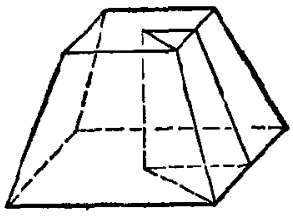
\includegraphics[width=4cm]{../pic/ltjh-ch2-21.png}
        \caption{}\label{fig:ltjh-2-21}
    \end{minipage}
    \qquad
    \begin{minipage}[b]{7cm}
        \centering
        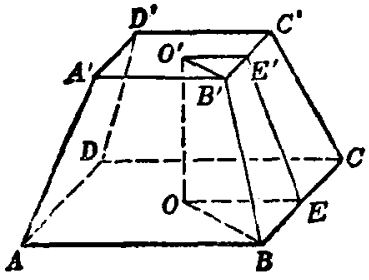
\includegraphics[width=5cm]{../pic/ltjh-ch2-22.png}
        \caption{}\label{fig:ltjh-2-22}
    \end{minipage}
\end{figure}

\liti 正四棱台 $AC'$ 的高是 17 cm,两底面的边长分别是 4 cm 和 16 cm,求这个棱台的侧棱的长和斜高(图 \ref{fig:ltjh-2-22})。

\jie 设棱台两底面的中心分别是 $O'$ 和 $O$,$B'C'$ 和 $BC$ 的中点分别是 $E'$ 和 $E$。
连结 $O'O$、$E'E$、$O'B'$、$OB$、$O'E'$、$OE$,则 $OBB'O'$ 和 $OEE'O'$ 都是直角梯形(图 \ref{fig:ltjh-2-22})。

$\because$ \quad $A'B' = 4$ cm, \quad $AB = 16$ cm,

$\therefore$ \quad \begin{zmtblr}[t]{}
    $O'E' = 2$ cm, \quad $OE = 8$ cm, \\
    $O'B' = 2\sqrt{2}$ cm  \quad $OB = 8\sqrt{2}$ cm。
\end{zmtblr}

因此 $B'B = \sqrt{17^2 + (8\sqrt{2} - 2\sqrt{2})^2} = 19 \;(\limi)$,

$E'E = \sqrt{17^2 + (8 - 2)^2} = 5\sqrt{13}\;(\limi)$。

\hspace*{-2em}即 \quad 这个棱台的侧棱长是 19 cm,斜高是 $5\sqrt{13}$ cm。


\liti 设棱台的两底面积分别是 $S$、$S'$,它的中截面的面积是 $S_0$。
求证: $2\sqrt{S_0} = \sqrt{S} + \sqrt{S'}$(图 \ref{fig:ltjh-2-23})。

\zhengming 因为棱台的中截面与两底面平行,所以多边形 $ABCDE$、$A_0B_0C_0D_0E_0$、$A'B'C'D'E'$ 相似。因此
$$ \dfrac{S}{S_0} = \dfrac{AB^2}{A_0B_0^2} \douhao \quad \dfrac{S'}{S_0} = \dfrac{A'B'^2}{A_0B_0^2} \douhao $$
也就是
$$ \dfrac{\sqrt{S}}{\sqrt{S_0}} = \dfrac{AB}{A_0B_0} \douhao \quad \dfrac{\sqrt{S'}}{\sqrt{S_0}} = \dfrac{A'B'}{A_0B_0} \juhao $$

将上面等式两边分别相加,因为 $A_0B_0$ 是梯形 $ABB'A'$ 的中位线,

$\therefore$ \quad $\dfrac{\sqrt{S} + \sqrt{S'}}{\sqrt{S_0}} = \dfrac{AB + A'B'}{A_0B_0} = \dfrac{2 A_0B_0}{A_0B_0} = 2$。

由此得到
$$ 2\sqrt{S_0} = \sqrt{S} + \sqrt{S'} \juhao $$

\begin{figure}[htbp]
    \centering
    \begin{minipage}[b]{7cm}
        \centering
        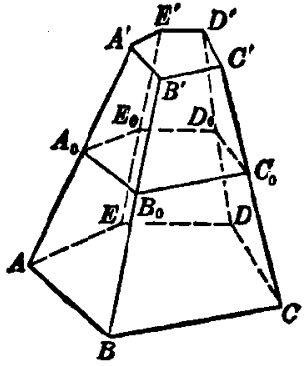
\includegraphics[width=5cm]{../pic/ltjh-ch2-23.png}
        \caption{}\label{fig:ltjh-2-23}
    \end{minipage}
    \qquad
    \begin{minipage}[b]{7cm}
        \centering
        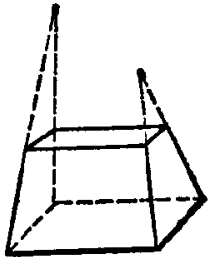
\includegraphics[width=3cm]{../pic/ltjh-ch2-subsec3-lx1-01.png}
        \caption*{(第 1 题)}
    \end{minipage}
\end{figure}


\begin{lianxi}

\xiaoti{图中的几何体是不是棱台?为什么?}

\xiaoti{一个正四棱台上、下底面的边长分别是 $a$ 和 $b$, 高是 $h$。 求经过相对的两条侧棱的截面面积。}

\end{lianxi}



\subsubsection{正棱台直观图的画法}

以正四棱台为例,说明正棱台的画法。

\begin{figure}[htbp]
    \centering
    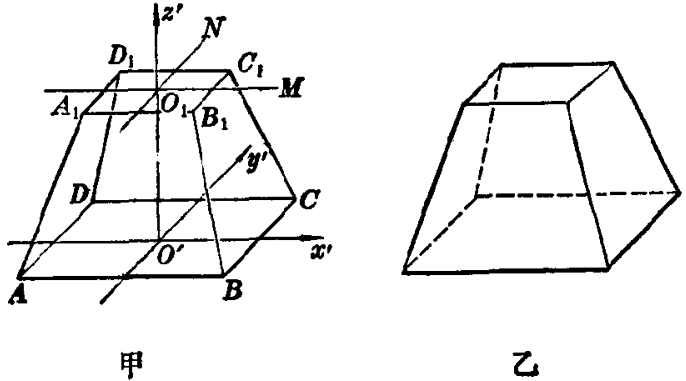
\includegraphics[width=10cm]{../pic/ltjh-ch2-24.png}
    \caption{}\label{fig:ltjh-2-24}
\end{figure}

\huafa (1)画轴 \quad 画 $x'$轴、$y'$轴、$z'$ 轴,使 $\angle x'O'y' = 45^\circ$, $\angle x'O'z' = 90^\circ$(图 \ref{fig:ltjh-2-24} 甲)。

(2)画底面 \quad 以 $O'$ 为中心,按 $x'$ 轴、$y'$ 轴画正四棱台下底面正方形的直观图 $ABCD$。
在 $z'$ 轴上取线段 $O'O_1$ 等于正四棱台的高。过 $O_1$ 画 $O_1M$、$O_1N$ 分别平行于 $O'x'$、$O'y'$,
再以 $O_1$ 为中心,按 $O_1M$、$O_1N$ 画正四棱台上底面正方形的直观图 $A_1B_1C_1D_1$。

(3)成图 \quad 连结 $AA_1$、$BB_1$、$CC_1$、$DD_1$,并加以整理,就得到正四棱台的直观图(图 \ref{fig:ltjh-2-24} 乙)。



\subsubsection{正棱台的侧面积}

棱台的侧面展开图是由各个侧面组成的,展开图的面积就是棱台的侧面积。正棱台的侧面展开图如图 \ref{fig:ltjh-2-25} 所示。
设它的上、下底面边长是 $a'$、$a$,边数是 $n$,斜高是 $h'$,
那么它的侧面积是 $n \cdot \exdfrac{1}{2} (a + a') h' = \exdfrac{1}{2} (na + na') h'$,
由于 $na'$、$na$ 分别是上、下底面的周长 $c'$、$c$,我们得到下面的定理:

\begin{dingli}[定理][dl:zlt-cmj]
    如果正棱台的上、下底面的周长是 $\bm{c'}$、$\bm{c}$,斜高是 $\bm{h'}$,那么它的侧面积是
    \begin{center}
        \framebox[14em]{$\bm{S_\text{正棱台侧} = \exdfrac{1}{2} (c + c') h'}$。}
    \end{center}
\end{dingli}


棱台的全面积等于它的侧面积与上、下底面积的和。


\begin{figure}[htbp]
    \centering
    \begin{minipage}[b]{7cm}
        \centering
        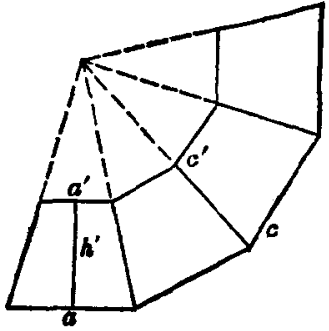
\includegraphics[width=5cm]{../pic/ltjh-ch2-25.png}
        \caption{}\label{fig:ltjh-2-25}
    \end{minipage}
    \qquad
    \begin{minipage}[b]{7cm}
        \centering
        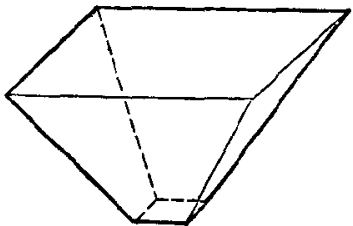
\includegraphics[width=5cm]{../pic/ltjh-ch2-26.png}
        \caption{}\label{fig:ltjh-2-26}
    \end{minipage}
\end{figure}


\liti 粉碎机上的下料斗是正四棱台形(图 \ref{fig:ltjh-2-26}),它的两底面边长分别是 80 mm 和 440 mm,高是 200 mm。
计算制造这样一个下料斗所需铁板的面积(保留两位有效数字)。

\jie 上底面周长 $c' = 4 \times 80 = 320$ (mm),

\qquad 下底面周长 $c = 4 \times 440 = 1760$ (mm),

斜高 $h' = \sqrt{200^2 + \left(\dfrac{440 - 80}{2}\right)^2} \approx 269\;(\haomi)$,

$\therefore$ \quad $S_\text{正棱台侧} = \exdfrac{1}{2} (c + c') h' = \exdfrac{1}{2} (320 + 1760) \times 269 \approx 2.8 \times 10^5 \; (\pfhm)$。

答:制造这样一个下料斗需铁板约 $2.8 \times 10^5 \; \pfhm$。


在正棱台的侧面积公式中,
如果设 $c' = c$,就得到正棱柱的侧面积公式: $S_\text{正棱柱侧} = ch'$(这里 $h'$ 是高)。
如果设 $c' = 0$,就得到正棱锥的侧面积公式: $S_\text{正棱锥侧} = \exdfrac{1}{2} ch'$。
这样,正棱柱、正棱锥、正棱台的侧面积公式之间的关系可表示如下图。

\begin{figure}[htbp]
    \centering
    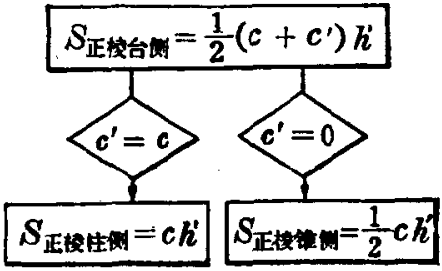
\includegraphics[width=7cm]{../pic/ltjh-ch2-subsec3-gsgx.png}
\end{figure}


\begin{lianxi}

\xiaoti{画出上、下底面边长分别是 2 cm 和 8 cm,斜高是 4 cm 的正四棱台的直观图。}

\xiaoti{一个正三棱台的两个底面的边长分别等于 8 cm 和 18 cm,侧棱长等于 13 cm。求它的侧面积。}

\end{lianxi}



\subsubsection{多面体}

前面,我们研究过的棱柱、棱锥、棱台,它们都是由一些多边形围成的几何体。
由若干个多边形所围成的几何体,叫做\zhongdian{多面体}。
围成多面体的各个多边形叫做\zhongdian{多面体的面},两个面的公共边叫做\zhongdian{多面体的棱},
若干个面的公共顶点叫做\zhongdian{多面体的顶点}。
许多矿物结晶体,例如食盐、明矾、石膏等都是呈多面体形的(图 \ref{fig:ltjh-2-27})。

\begin{figure}[htbp]
    \centering
    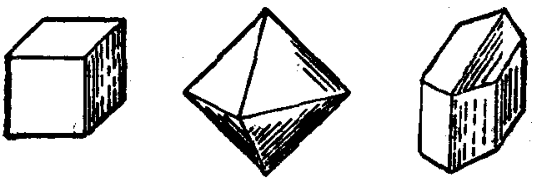
\includegraphics[width=9cm]{../pic/ltjh-ch2-27.png}
    \caption{}\label{fig:ltjh-2-27}
\end{figure}

把多面体的任何一个面伸展为平面,如果所有其他各面都在这个平面的同侧,这样的多面体叫做\zhongdian{凸多面体}(图 \ref{fig:ltjh-2-28})。

\begin{figure}[htbp]
    \centering
    \begin{minipage}[b]{7cm}
        \centering
        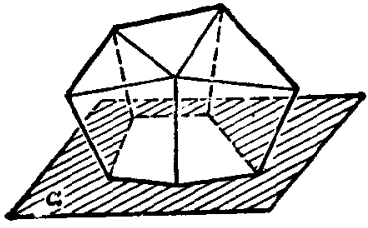
\includegraphics[width=5cm]{../pic/ltjh-ch2-28.png}
        \caption{}\label{fig:ltjh-2-28}
    \end{minipage}
    \qquad
    \begin{minipage}[b]{7cm}
        \centering
        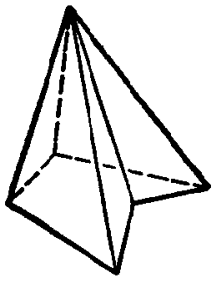
\includegraphics[width=3cm]{../pic/ltjh-ch2-29.png}
        \caption{}\label{fig:ltjh-2-29}
    \end{minipage}
\end{figure}

前面研究过的所有的棱柱、棱锥、棱台指的都是凸多面体。 图 \ref{fig:ltjh-2-29} 中的多面体不是凸多面体。

一个多面体至少有四个面。多面体依照它的面数分别叫做\zhongdian{四面体}、\zhongdian{五面体}、\zhongdian{六面体}等。
例如,三棱锥是四面体,三棱柱是五面体,正方体是六面体等。


\begin{lianxi}

\xiaoti{图示多面体、凸多面体、棱柱、棱锥、棱台、平行六面体各集合的包含关系。}

\xiaoti{在学过的一些多面体中,举出五面体、六面体、七面体的例子,除三棱锥外,还有四面体吗?}

\end{lianxi}

\end{enhancedline}

